% Chapter 1

\chapter{Introduction: A Better Time-Based Installation} % Main chapter title

\label{Chapter1} % For referencing the chapter elsewhere, use \ref{Chapter1} 

\lhead{Chapter 1. \emph{A Better Time-Based Installation}} % This is for the header on each page - perhaps a shortened title

%----------------------------------------------------------------------------------------
%	Abstract
%----------------------------------------------------------------------------------------
\section{Introduction}

What constitutes good design? As expressed by Don Norman in the book "The Design of Everyday Things," design can be sympathetic to their users, or have psychopathy coded directly into their construction. ScreenPerfect has been designed to address the question of how we might improve software based on internet technologies to be more useful to artists.

This project has several parts, which will be explained separately. The first part of the project is an application to build branched narratives out of video files, coded in NodeJS for distribution via common internet technologies. This portion of the research has to do with the idea of resistance and how people's consciousness and abilities can be expanded by using contemporary technology, which is made by trained technicians but then released to be used without a proscriptive definition of the use case. Users make use of the engine, developed through one specific user's design practice, to design new things. The first part addresses the importance of this type of engine to generation of contemporary art experiences.

The second part of this paper addresses how to perform user testing via a game jam format, a type of design charette in which users are given access to tools and asked to produce art with them. In that section, I document how No Jam 2: videovideo worked, the industry paired advantages to new engine development, and how this expands community ties for local artists working in a medium that frequently demands more collaboration than traditional, less dynamic art works.

In the third part of this paper, I address the issue of new media art and display. New media, particularly time-based media, is very challenging to display and support. Even low-end computers are bulky and expensive to deploy, so I have asked the question of how we might circumvent traditional white-cube galleries while restricted by the requirements of internet technologies. In this part I detail how to build a server on the raspberry pi platform, a microcomputer, to deploy web-based applications to localized, internet-restricted spaces. 

In conclusion, I argue that we need technology to belong to its users, instead of pursuing an exclusive reliance on mass network technologies. I feel that there has always been room for the technical in art, and while good technology fades into the background to leave only the artwork on display, the technology we choose to use gives us a frame of what can be pursued. 

%----------------------------------------------------------------------------------------
%	Tech to video art to video games text to video games video
%----------------------------------------------------------------------------------------

\section{Designing Software to Power Experience}
The arts and the humanities are the technical name for the fields of work that produce both North America’s culture and its record of its culture. We use computers to do the work, because they extend our ability to speak in repeatable patterns. Repetition is a key component of mass production. Looked at as a tool, a computer is not so much a hammer as it is an ongoing negotiation - the user must decide what the black box means \cite{glanville}.

The use of computers as tools is a specific skill set, which is as unique as the skill set of using a paintbrush. The key element of computer skills is a comfort with curiosity: digital tools change all the time, and many of them are not well written. Software is frequently unreliable, and hardware moreso. Almost all software tools require a vast period of time invested in skill acquisition before content - art - can be produced, and this time is expensive. The construction of the tools themselves is an art, because when manufacturing a tool, it needs to be easily used, but it also needs to do something in a predictable, reliable way. A good digital tool should encourage rather than impede expression. 

Artists, as a rule, have their own working methods and vision for their work in advance of picking up any new tool. For the purposes of this work, it is assumed that users have their own vision independent of the tool itself, which can be expressed, expanded, or extended by the use of a new tool. Ideally, a tool vanishes in its use. It is a multiplier of force, where force can also be capital, which can be either an intellectual weight - the gravity of a cultural construct distending other expressions - or the more conventional "money."

Television and video are a format requiring intense capital to access. Culturally, video works - film, television - express mass ideals to mass audiences. YouTube, Vimeo, the late Steve Job's well-documented interest in the format, and visual FX production continue to drive technological innovation in systems development. Most movies have some vFX to them, a capital-intense practice that requires hours of work. Acquiring editing skills and image-design skills to work with moving pictures is an expensive and time-consuming pursuit, which has nonetheless become more open in recent years. The advent of Vine and YouTube has democratized video to the point where it can be traded as words once were.

This does not make the expression of capital inherent to these works more valuable, but less. It becomes apparently disposable, consumable on devices that are as close to us as clothing. Video is consumable on every kind of screen, especially on the smartphone screen. On one level, this is great for audience acquisition. On another level, it shifts the import of the work from the work to the container. Though the medium has been the message, in the contemporary internet, the envelope is the note.

Fortunately, in the contemporary internet, the envelope is also the entire postal service. A single smartphone in 2014 is more than powerful enough to supply most of the switching and serving needs of previous video works, including branched narratives that once required many VCRs and multiple screens. As things become more accessible, they lose their Walter Benjamin aura, their singular magic, which means that accessing that magic becomes more challenging as the distribution of the work becomes easier. Partly, this seems to be a process of decontextualization: no matter how good a given film, it may be better in a theatre, en masse, because the theatre, the production of context and attendance, makes the experience of the film singular, even as the film itself is limitlessly reproducible.

So the question becomes: how to best retain the capital of artistic tool use, vision, and creative practice, while restoring the aura of presentation required to engage with art on its own terms? How to expand artistic tool use into new means of expression? How to make use of contemporary methods in a way that may remain accessible and on display for years to come? 

%----------------------------------------------------------------------------------------
%	Interaction and Presentation
%----------------------------------------------------------------------------------------
\section{Interaction and Presentation in Game Design}

Games, particularly the subset of video games known as triple-A, are expensive to make and practically require a team of people to produce. This has been seen as restricting the degree to which the stories these experiences communicate can be personalized. While there are counter-examples, such as 2013's excellent "Saint's Row 4," many triple-A games need to be able to make back their budget, which restricts their intended audience to those who can pay to play. The games themselves utilize engines which are generally private or closed-source. An engine is the software that dictates how the physics and scripting that contains a game world can be manipulated. Many are closed-source and privatized, and therefore expensive. All of the engines as they presently exist require not only the skill of framing and lighting an engaging experience, but also a panoply of other skills - character modelling, animation, colour theory, programming or scripting, and sound.

This creates a design challenge: How to best reduce the barriers to entry in game-making to encourage new voices?

A new type of game engine is one possible approach. An engine is the body of software that drives all interactions in-game. Assets, such as artwork, music, animations, and scripts to dictate how these assets are integrated, are all added to an engine that provides a framework to drive any given game. Some engines encourage more experimentation than others. The Twine engine, for example, is designed to provide branched, highly-stylized text narrative to a web browser, and it has been adopted by its userbase to tell detailed stories that are highly personal - the sort of work that cannot always be addressed by games with a bigger budget. Twines are limited in form but not in scope. The Unity engine provides traditional assets and scripting, and has been used by independent developers to produce games such as Gone Home (2013), a work about a missing family mainly told through examining objects and listening to music. Twine takes advantage of an author's skill at pacing and writing to divide a narrative into a choose-your-own-adventure work, paced through timed links and designed to take advantage of the detailed design possibilities of text in the browser.

Independent games are typically distributed through the internet, or rely on the internet for their entire lifecycle. This is problematic, not only because the shape of the engine dictates the shape of the experiences that can be produced. The internet is owned, mainly, by very few extremely wealthy people, and the technology is fragile. There are many ways to lose access, from legal means such as France's HADOPI laws, by which whole households can have their access cut off, to a simple lack of bandwidth in an installation space. This causes huge problems for both exhibitions and archives, as art based on access to the external web can vanish with no warning. This is also unacceptable for institutional collection. The availability of web art combined with its unreliability devalues the work of the artists who have created it. Art that relies on the network is simultaneously omnipresent and vanishing, capable of accessing a mass audience and disappearing at the moment when a local audience is available.

Audience definition becomes important in this context. A browser-based or internet-distributed game has the possibility of reaching a very broad audience - millions of users. The artist has no guarantee of the context of their work in the view of the audience, beyond that it is likely to be screen-based, viewed on a personal or work machine. Perhaps this works. Whether or not screen-based art as it presently exists is effective is outside the scope of this paper, however. Within the scope of this work is that digital work is difficult to display \textit{outside} the context of this mass market.

If electronic art is to be included in large collections, or displayed privately, or reproduced such that it benefits mainly the artist rather than the distributor, there needs to be a means to display it that does not rely on external resource providers. This includes the easily-considered difficulty of network providers as well as the more challenging to contextualize power grid. Both are unreliable in the permanent sense, where the relatively small amounts of power and information (which are sometimes the same things) can actually be supplied locally. 

The localization of a broad audience - how to supply a thousand or ten thousand people simultaneously with a single experience - is outside the scope of this paper. This design work instead addresses the question of how to bring a work built for broad distribution into a narrow context for better engagement via a system of resilient display. This system uses local resources rather than relying on global supply to always be there.

This touches on themes of paranoia, privacy, and the resistance techniques beloved of both cybernetics and French post-structural feminism. There is a sense of play in code: there are many, many ways to achieve a topically identical personal experience using software.

Web technology is important to software development for a variety of reasons, part of which is that it is already more accessible to novice users than traditional, desktop compiled software. Web browsers have offered users the ability to view the source code of the pages that users are reading, which includes the content of scripts. With the advent of developer tools included standard in browsers, it has become straightforward to build and test software ideas quickly in an environment provided on every operating system. This is now under threat with the advance of embedded digital rights management software \cite{arstechnicadrm}, but it remains an important learning resource, because it is available with every desktop computing platform.

People who have little time cannot afford to acquire the skills to use a new and complex tool. Due to these restrictions, the number of people for whom computer use in and of itself will be a delight is a limited population. This is problematic, because art production is difficult and time-consuming even without the boundaries raised by software challenges. The more limited and specific the skill set required to use contemporary software tools, the more difficult it is to include a diversity of voices in the cultural production of genuinely contemporary work. When artists are excluded from technology, culture splits on lines of privilege. There are artists who make art, and technologists, who make technology, but do not see themselves as particularly responsible for the ideas encoded in their work. 

Technology is not neutral. It is authored, and where there is authorship, there is a responsibility for ideas. When large groups are left out of communication media, particularly those tasked with producing the language with which culture speaks to itself, there comes a disconnect in the public representation of our sense of self. 

The problem of interesting experiences is not trivial. Video games offer an economically advantageous distraction engine, a way to enact an artificial life during a period of declining general wealth. Allowing a diverse range of voices easy access to portray their own games, their own alternate or idealized modes of being, is a way of making those voices more real, of offering an alternate human experience to the “asshole simulator” (\cite{bissell}) genres manufactured at much higher budgets.


\section{Initial Approach}


\subsection{Federal Development Grant, game::play Lab, and collaborative artistic practices}

The initial code of screenPerfect came about as part of a collaborative development project in OCADu's game::play lab to produce a vision of how dual-screen artworks might work going forward. The original software powered a game called psXXYborg, produced by Hannah Epstein under the supervision of Emma Westecott. From there, I became curious as to how we could transform the engine software to include game-editing tools, to encourage a wider range of video artists to use the software. This became the basis of the initial portion of my thesis work, the screenPerfect engine. In order to generate sufficient games to demonstrate the software, and to figure out where the software could be improved, we then partnered with Bento Miso coworking space in a mutually beneficial game jam called No Jam 2.

No Jam 2 featured both an editing segment and a re-architected version of screenPerfect that uses Bento's new language, Daimio, designed mainly for open use on the internet. After the jam, the games were collected, with their resources, and screenPerfect was forked to become two separate engines. The original engine was retained for displaying works to that point, and a new engine called iV to promote ease of access within the Dames Making Games, a feminist social group run at Miso by the same developers who worked on the engine. 

iV differs from screenPerfect in that it drops the dual-screen element and encourages a single-focus narrative. ScreeenPerfect has also been reoptimized for local display of static files from a single Linux-based computer. I selected a raspberry Pi, both because of its scale and affordability, and because it stems from a collaborative learning foundation in the UK.

There is no part of this work which is not an assembly of other works, which does not rely on the network of the internet being at least in part an open place to learn how to build software. This is an essentially agile, iterative development process, wherein the first type of software was delivered, and everything that has emerged afterwards has been an evolution of the initial design concepts, which were themselves an end goal. This is programming from back to front - hacking, in Sadie Plant's definition, a practice where one starts at the end of what one is looking for and then sews up every step on the way until the software works as intended \cite{plant}. This type of systems design is holistic, borrowing heavily from independent game design and general creative practice.

The formal agile method of software development is based on the idea of delivering working code in advance of documentation, and putting the user ahead of the planner in software design. I have included a summary of the method in Appendix A, The Agile Manifesto, but what it chiefly means is less advance software planning of every detail, and more asking questions about the best way to solve a problem in code. 

This thesis assumes that the definition of gaming as an art form dependent on action (\cite{galloway}) is accurate, and therefore, after developing an initial round of software, the main body of feedback and development in this software package has been via user collaboration. The volunteers can then give feedback to both the software developers and to each other on what is possible with the tool. At that point, I will incorporate their feedback into future versions of the tool, hopefully leading to a stable platform for interactive experience development. This is a dynamic type of user-centered design, relying heavily on version tracking software and rapid updates, in line with agile development ideals.

The initial software underlying screenPerfect has been developed in concert with an artist who laid out an idea for how a video interaction might work, which has then been created and refined, released to more artists, and then revised again. The hope is that each new version of the tool will generate a useful echo chamber, amplifying new ideas even as it makes advanced technology easily accessible to content producers.

The toolset can then be released and left for artists to use and analyse, and can be expected to run privately on optimized systems similar to "game cartridges" from the 1990s. 
\begin{figure}[h!]
 \caption{Game Cartridge of Chrono Trigger, 1995}
  \centering
    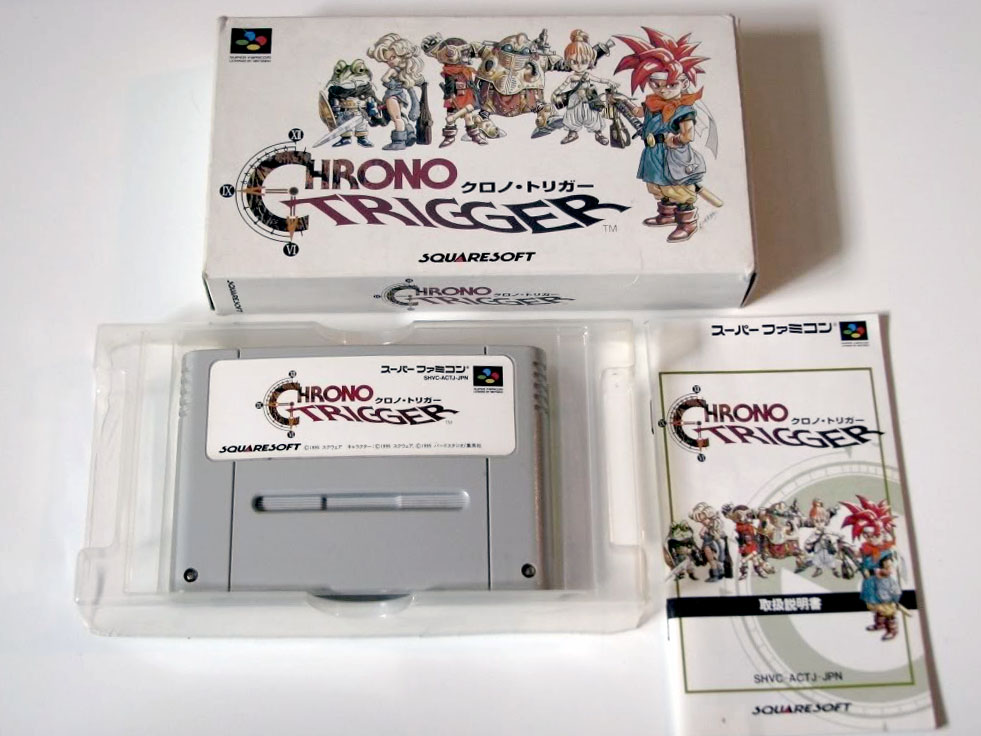
\includegraphics[width=0.5\textwidth]{gamecart}
\end{figure}

\subsection{Code and Theory}

The initial software of this project was developed as a response to the lack of privacy and control of various shared media sources online. Rather than developing for a mass audience, I began with the idea that this should be developed privately, for small audiences using disconnected technology. Over the course of many installations of the psXXYborg software package, I noticed many installation issues, many dependent on a reliance on external resources.

The code of screenPerfect was written in Javascript on the server and client side, using Node.JS. Node is a server environment library and framework that is intended to permit web developers familiar with JS to write their code to the server. During the process of the thesis, the idea of screenPerfect as a game engine was taken up by my industry partners, Bento Miso, who are interested in the idea of new game engines as a use case for their language, Daimio (\cite{daimio}). In the case of ScreenPerfect, I decided to write the initial application in Node.JS and javascript to take advantage of the speed of the Google V8 code engine. When that application was done, I turned it over to Miso, who refactored the code into something that could be attached to the Daimio language system.

The critical theory that underlies this practice is a combination of French poststructuralism - Helene Cixous in particular - and contemporary writing on video games and the history of women in technology. By producing the software and content with the input of a local feminist collective, Dames Making Games, I have grounded the work in a social justice driven practice which encourages women to take part in their own lives by learning how to interact with machines and communicate with the broader world.

\subsection{Game Engine Research}

The Twine engine is a branching narrative engine for authoring text narratives. I have taken the idea of Twine and transformed it to use video and still images to expand the possibilities of an author experience.Twine is affordable and requires very little training to access, but it is also limiting, in that it undermines skillsets in imagemaking which may already be highly realized. 

Video games, particularly console-based video games, have a huge leg up on experimental art in one basic respect. Video games are still generally expected to run when the internet vanishes. The Nintendo 3DS, a pocket console, outsold every other system on the market in 2013 \cite{nintendosales}. It is speculated that its success is due largely to the fact that the 3DS is a portable system that does not connect to the broader internet unsupervised. You purchase games for it on cartridges, which contain that piece of software and no others. This makes the system portable, unlikely to be co-opted by malware, and controllable, in that it is tough to get to the wilder areas of the internet unsupervised. This reliability is something that is rare to find in more complex computers: sometimes, as argued by Don Norman in "The Design of Everyday Things" \cite{norman}, it is best to have a single thing do one thing really well. 

Cartridge design is excellent, and limited. Cartridges historically fit into one system, once, and rely on details of that system's hardware to run. They still run on their original hardware as much or more than twenty years later, provided the original hardware can be kept to spec, where newer software, reliant on repeated patching after launch, may fail more frequently.

The other good example of portable electronic interaction is the smartphone. Mobile is a huge segment of the market, which is excellent for text messaging, talking, and playing games that separate an audience from each other, but not so great for bringing people together in the same space. Part of the appeal of the smartphone is that it is \texit{customizable}, which means that each user can design their own experience and use it. 

There are games that choose to subvert this separation, and systems have been built to take advantage of the power of pocket computers. The most notable effort to date is "Space Team," a simon-says game for teams of up to four players. The application pairs to itself across phones by using a common network connection, and players in the same physical space cooperate to pilot a star ship. This is excellent, as it allows players to make use of a device with which they are already comfortable to cooperate and share an experience.

Unfortunately, it is limited to Apple users, because SpaceTeam is an application, limited to a single system.

The idea underlying screenPerfect is that all users have access to the internet on their pocket devices, and the internet is both bigger and smaller than the network which delivers content to users. Rather than relying on The Internet, screenPerfect provides a private wiFi point and what is called a "captive portal" to let players pair with one another and the server, control a large screen, and interact with a piece of video art in a localized area. This means that an artist can control the exhibition space for their work, design the experience of the work, and ensure that their audience will experience the work in a context that makes sense. It aso ensures that technicians can access the underlying engine should something go wrong during the installation.


\subsection{Experiments in System Control within Cybernetics and Feminism}

This work is related to various texts of feminist or woman-oriented critical theory that have appeared in the years since: Haraway’s Cyborg Manifesto, TIQQUN’s Preliminary Materials Towards A Theory of the Young-Girl. These are academic constructions of femininity as it is seen in relation to technology: they are feminist in the formal sense of the word. There are other senses of the term, which I will not be examining within the paper. Rather than expressing this work in context with Cixous as \textit{écriture feminine}, I will be using Cixous as a reference for the idea of the alien perspective as a position of resistance within a means of expression controlled by a neutral-to-hostile majority. 

This approach addresses women as an alien construct to the more conventional world of technology, which has been recently associated with a masculinist performance that is unnecessary for the pure structure of good rules and the development, through that, of good software. This construction is relatively recent, as Nathan Ensmenger presents within his work on the systematic exclusion of women from programming as a trade (\cite{ensmenger}).

Accessibility for artists is a major contemporary concern, related to the development of languages like Processing by Ben Fry and Casey Reas (\cite{processing}), microcontrollers like the Arduino platform by Massimo Banzi &co. (\cite{arduino}), and frameworks like Scratch from the MIT Lifelong Kindergarten Group (\cite{scratch}). 

People who write code to develop an idea are engaging in a conceptual creative practice themselves, and they then display that creative practice through the artists who use their work. Purposefully producing small tools to support creative practice is a different model than that of major software development houses, where the work is designed in isolation, iterated on a strict schedule - 18 months in the case of Adobe \cite{adobe} - and released. There are documented design methods for software that follows this model - I have listed Agile as the most well-known - but for the most part, this is simply considered an interative working practice which aims to a functional, finished result.

Although artists are the central agents of production of the invisible yet tangible value of the culture industry, they are not the prime beneficiaries of the financial system that backs, stores, and distributes the results of that capital. This is capital as both skill and capital as resource distribution: computers are expensive. Getting around that face is important if we wish to supply access to contemporary media to a broad array of voices: to be inclusive, software should be the last thing that gets in the way of a work, rather than the first. This reserves the value of scarcity - the market value of the work - to the \textit{ability} of the artist, rather than applying the majority value to the role of the engineer. This kind of invisibility is the invisibility of good management, of any type of good administration. Like housekeeping, code recedes until something goes wrong.

To test this idea, I have approached people to produce video|games with the screenPerfect software in the context of a voluntary game jam – a type of collaborative space where participants work with digital tools to generate new, raw games in a limited window – and then compiling the results into an arcade machine for presentation. 
